\chapter{Description}
\section{Problem Statement}
\begin{itemize}
\item The objective of the project is to overcome the disadvantages present in the existing system.
\item Provide tailor made services to accommodate dynamic parameters of the university.
\item Provide tailor made services to the needs of institute.
\item Bridging gap between manual human work flow to digital work flow.
\end{itemize}
\section{Features of Proposed System}
\begin{itemize}
\begin{figure}[ht]
\centering
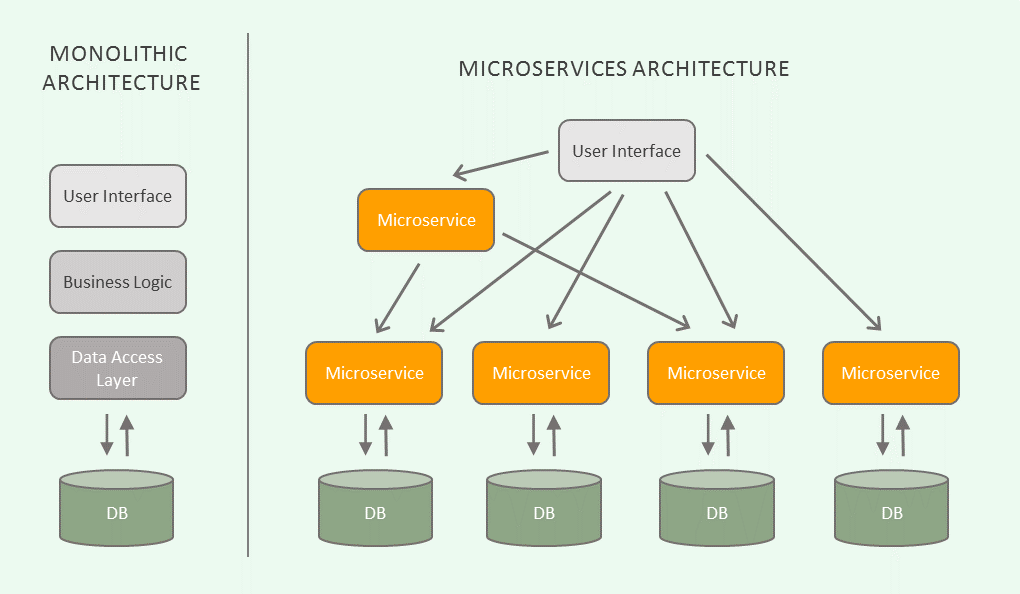
\includegraphics[width=35em]{figures/figure2.png}
\caption{Mono Lithic v/s Micro Service Architecture}
\end{figure}
\item \textbf{Microservice Architecture}\par
Microservices are a software development technique —a variant of the service-oriented architecture (SOA) structural style— that arranges an application as a collection of loosely coupled services. In a microservices architecture, services are fine-grained and the protocols are lightweight.
\begin{figure}[ht]
\centering
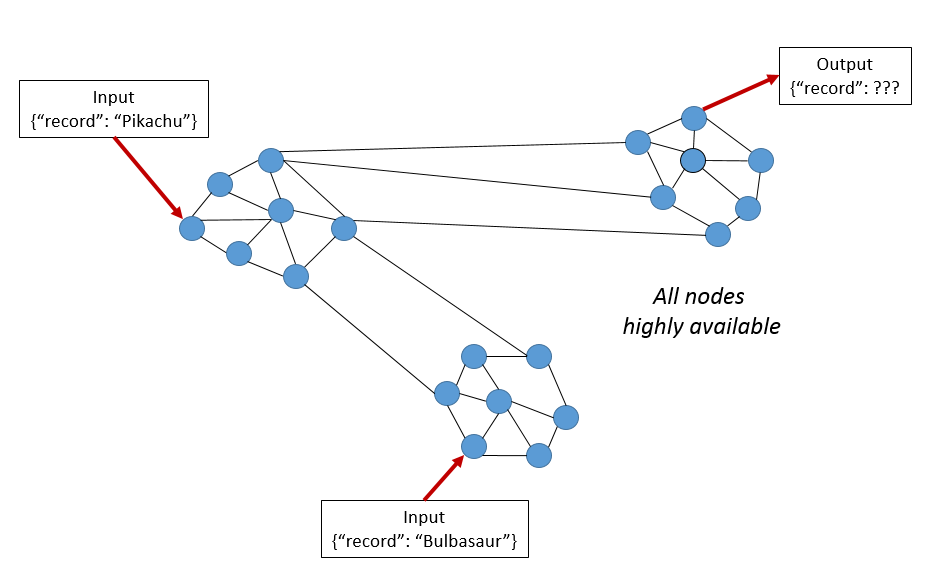
\includegraphics[width=35em]{figures/figure3.png}
\caption{Distributed System Architecture}
\end{figure}
\item \textbf{Distributed System}\par
Distributed computing is a field of computer science that studies distributed systems. A distributed system is a system whose components are located on different networked computers, which communicate and coordinate their actions by passing messages to one another. The components interact with one another in order to achieve a common goal. Three significant characteristics of distributed systems are: concurrency of components, lack of a global clock, and independent failure of components. Examples of distributed systems vary from SOA-based systems to massively multiplayer online games to peer-to-peer applications.
\par
A computer program that runs within a distributed system is called a distributed program (and distributed programming is the process of writing such programs). There are many different types of implementations for the message passing mechanism, including pure HTTP, RPC-like connectors and message queues.
\par
Distributed computing also refers to the use of distributed systems to solve computational problems. In distributed computing, a problem is divided into many tasks, each of which is solved by one or more computers, which communicate with each other via message passing.
\begin{figure}[ht]
\centering
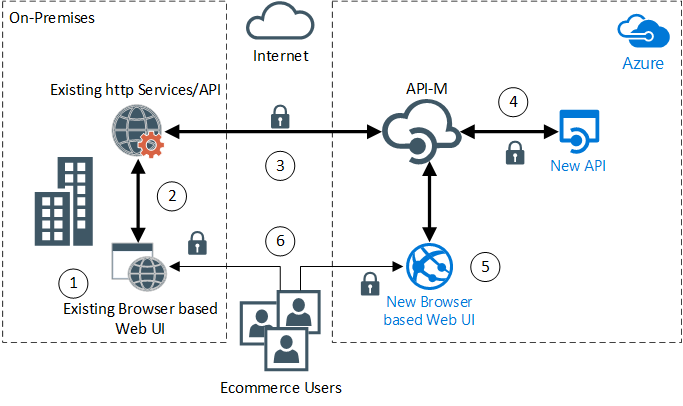
\includegraphics[width=35em]{figures/figure4.png}
\caption{API System Architecture}
\end{figure}
\item \textbf{API Oriented}\par
An application programming interface (API) is an interface or communication protocol between a client and a server intended to simplify the building of client-side software. It has been described as a “contract” between the client and the server, such that if the client makes a request in a specific format, it will always get a response in a specific format or initiate a defined action.
\par
An API may be for a web-based system, operating system, database system, computer hardware, or software library.
\par
An API specification can take many forms, but often includes specifications for routines, data structures, object classes, variables, or remote calls. POSIX, Windows API and ASPI are examples of different forms of APIs. Documentation for the API usually is provided to facilitate usage and implementation.
\item \textbf{Cross Platform Development}\par
Cross-platform software (also multi-platform software or platform-independent software) is computer software that is implemented on multiple computing platforms. Cross-platform software may be divided into two types; one requires individual building or compilation for each platform that it supports, and the other one can be directly run on any platform without special preparation, e.g., software written in an interpreted language or pre-compiled portable bytecode for which the interpreters or run-time packages are common or standard components of all platforms.
\item \textbf{Role Based Security}\par
Role-based access control (RBAC) or role-based security is an approach to restricting system access to authorized users. It is used by the majority of enterprises with more than 500 employees, and can implement mandatory access control (MAC) or discretionary access control (DAC).
\par
Role-based access control (RBAC) is a policy-neutral access-control mechanism defined around roles and privileges. The components of RBAC such as role-permissions, user-role and role-role relationships make it simple to perform user assignments.

\item \textbf{Central Identity Management}\par
Identity management system refers to an information system, or to a set of technologies that can be used for enterprise or cross-network identity management.
\par
Additional terms are used synonymously with “identity management system” including;
\begin{itemize}
\item Access governance system
\item Identity and access management system
\item Entitlement management system
\item User provisioning system
\end{itemize}
Identity management (IdM) describes the management of individual identities, their authentication, authorization, roles and privileges within or across system and enterprise boundaries with the goal of increasing security and productivity while decreasing cost, downtime, and repetitive tasks.
\par
"Identity management" and "access and identity management" (or AIM) are terms that are used interchangeably under the title of identity management while identity management itself falls under the umbrella of IT security.
\par
Identity management systems, products, applications, and platforms are commercial Identity management solutions implemented for enterprises and organizations.
\par
Technologies, services, and terms related to identity management include active directories, service providers, identity providers, Web services, access control, digital identities, password managers, single sign-on, security tokens, security token services (STS), workflows, OpenID, WS-Security, WS-Trust, SAML 2.0, OAuth, and RBAC.
\begin{figure}[ht]
\centering
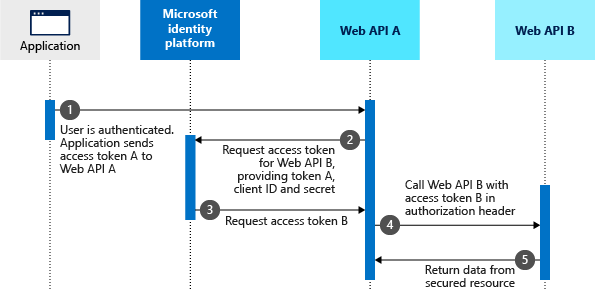
\includegraphics[width=35em]{figures/figure5.png}
\caption{OAuth 2.0 Flow}
\end{figure}
\item \textbf{Utilizes OAuth 2.0 Architecture}\par
OAuth is an open standard for access delegation, commonly used as a way for Internet users to grant websites or applications access to their information on other websites but without giving them the passwords. This mechanism is used by companies such as Amazon, Google, Facebook, Microsoft and Twitter to permit the users to share information about their accounts with third party applications or websites.
\end{itemize}
\section{Overview of Proposed System}
Capturing complete academic lifecycle of student into the system. Scopes of student’s application include:
\begin{itemize}
\item Attendance
\item Results
\item Library
\item Admissions
\item Fests
\item Availability of Staff
\end{itemize}
\par
Capturing complete journey of staff into the system. Scopes of staff’s application include:
\begin{itemize}
\item Communication
\item Attendance
\item Capture student data
\item Admissions
\item Leave Status
\item Calendar
\end{itemize}